\newpage
\section{Mögliche Aspekte}
\subsection{Persönliche mobile Arbeitsumgebung}
\subsubsection{Funktionalität}
Heutzutage werden Computer für alle möglichen Tätigkeiten in der Arbeitswelt benötigt, ob nun für kleinere Aufgaben oder für komplexe Berechnung mit Hilfe eines am Netzwerk angeschlossenen Supercomputers. In einer modernen Umgebung kann es unter Umständen notwendig sein den Arbeitsplatz aufgrund einer Tätigkeit zu wechseln um diese ausführen zu können. Dies hat allerdings zur Folge, dass dort der eigene Rechner mit den zugehörigen Daten und möglicherweise auch die benötigte Rechenleistung nicht verfügbar ist.
Um für die Benutzer eine auf allen Rechnersystemen einheitliche Bedienerfahrung gewährleisten zu können, lässt sich eine sogenannte mobile personalisierte virtuelle Computerumgebung (MOVE)\nomenclature{MOVE}{Mobile Personalized Virtual Computing Environment} nutzen. Durch diese Umgebung wird dem Benutzer auf jeder beliebigen Maschine eine gleichmäßig konsistente Desktop-Rechner-Umgebung präsentiert, welche sowohl die gleichen personenbezogenen Daten und Software als auch die verfügbare Rechenleistung liefert wie am eigenen Arbeitsplatzrechner. Eine solche Desktop-Rechner-Umgebung besteht zum Großteil aus der installierten Software einschließlich des Betriebs- und Dateisystems. Diese könnten zwar vom Speichermedium auf ein anderes übertragen werden, aufgrund der engen Koppelung ließe sich diese allerdings nicht einfach auf einem neuen System ausführen. Um diese Abstraktion gewährleisten zu können, wird die Technologie der virtuellen Maschinen (VM)\nomenclature{VM}{Virtual Maschine} genutzt.\footcite[Vgl.][Seite 890 f.]{MOVE}

Bei der Virtualisierung werden mit Hilfe von Technologien die Ressourcen eines Rechnersystems auf mehrere einzelne Klienten aufgeteilt um diese effektiver und flexibler nutzbar zu machen. Dies geschieht dadurch, dass unterschiedliche Klassen von Anwendungen auf wenigen physischen Systemen konsolidiert und von mehreren unabhängigen Betriebssysteminstanzen gleichzeitig genutzt werden können.\footcite[Vgl.][Seite 197]{InformatikSpektrum} Diese Virtualisierung wird mit der Hypervisor Technologie implementiert. Ein Hypervisor, oder auch Virtual Maschine Monitor (VMM)\nomenclature{VMM}{Virtual Maschine Monitor} genannt, ist ein Stück Hardware oder Software welches Systemressourcen virtualisiert, wobei zwischen Typ 1 und Typ 2 Hypervisors unterschieden wird. Typ 1 Hypervisors sind direkt auf der Hardware implementiert, Typ 2 Hypervisors laufen dagegen auf einem Host Betriebssystem. Dieses stellt Dienste wie Speichermanagement zur Virtualisierung zur Verfügung.\footcite[Vgl.][]{ibm}

\begin{figure}[H]
\begin{center}
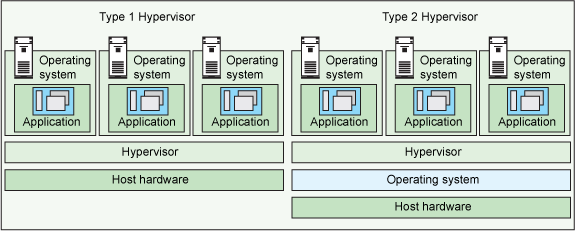
\includegraphics[width=0.9\textwidth]{hypervisors}
\caption{Unterschiede zwischen den Typ 1 und Typ 2 Hypervisors}
Quelle: \cite[]{ibm}
\end{center}
\end{figure}
\vspace{-1cm}

Solch ein zwischen Host-Hardware-Maschine und Gastsoftware implementierter VMM ermöglicht in diesem Fall die Koexistenz mehrerer Gastbetriebssysteme auf einer einzigen Single-Host-Hardwareplattform, indem eine vollständige Abstraktion von virtualisierten Hardwareressourcen zur Verfügung gestellt wird. Die Gastbetriebssysteme sind voneinander isoliert und können, entkoppelt und unabhängig von der zugrunde liegenden Hardware, auf dieser virtualisierten Plattform arbeiten. Die einzige Voraussetzung zur unmodifizierten Ausführung des Betriebssystems auf dem neuen Computer ist die Bereitstellung der gleichen virtuellen Plattform auf dem Zielsystem. Die Daten einer Computing-Umgebung lassen sich zusätzlich aufgrund der Speicherung des Dateisystems und des Software-Stacks beispielsweise als Image-Datei sehr einfach auf ein anderes System übertragen. Dies bedeutet, dass der VMM auf jedem davon unterstützten Gerät als eine einheitliche virtuelle Betriebssystemplattform dienen kann.\footcite[Vgl.][Seite 891]{MOVE}

\subsubsection{Aufbau eines MOVE Systems}
Ein MOVE System besteht im Großen und Ganzen aus vier Komponenten: einem MOVE Client, einem MOVE Server, privaten Netzwerkressourcen und einem IP Netzwerk. Das firmeninterne private LAN wird gebildet durch den MOVE Server und den übrigen privaten Netzwerkressourcen, der MOVE Client hingegen kann jede beliebige Maschine im Netzwerk sein und ist über das IP Netz mit dem privaten LAN verbunden. 
Der Nutzer zieht sich an einem beliebigen MOVE Client über das Netz eine lauffähige Instanz seiner eigenen Computing-Umgebung. Diese Instanz ist die persönliche virtuelle Computing-Umgebung. Die Daten des Benutzers werden durch seine Aktivitäten manipuliert, weswegen zur Erhaltung einer einheitlichen Umgebung auf allen Clients jede Operation zur Manipulation ebenfalls direkt auf dem MOVE Server ausgeführt werden muss. Dadurch wird gewährleistet, dass zu jeder Zeit an jedem Client der Benutzer die gleiche Umgebung erhält, die er zuvor verlassen hat.\footcite[Vgl.][Seite 891 f.]{MOVE}

\begin{figure}[H]
\begin{center}
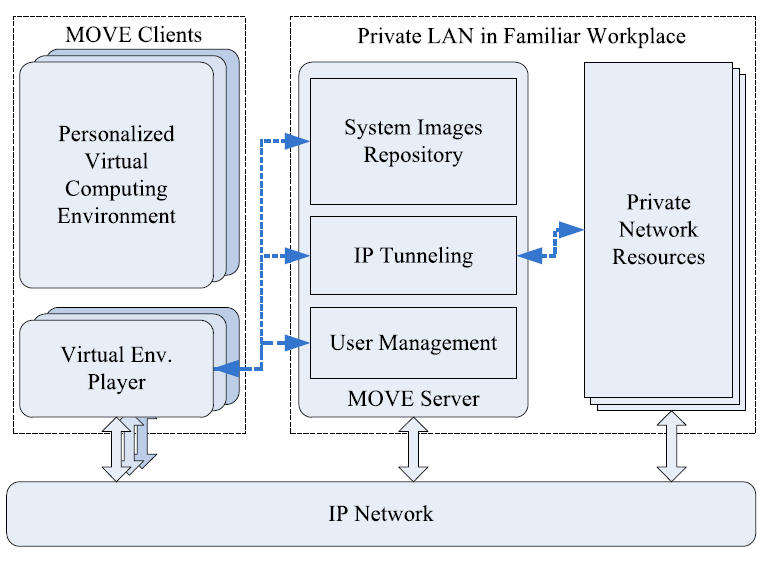
\includegraphics[width=0.9\textwidth]{move}
\caption{Komponenten einer MOVE Architektur}
Quelle: \cite[Seite 891]{MOVE}
\end{center}
\end{figure}
\vspace{-1cm}

Um diese Funktionalität zu ermöglichen sind einige Voraussetzungen notwendig. Zum einen wird für die Ausführung des persönlichen Desktops auf einem Client ein sogenanntes System Image benötigt. Dieses enthält alle Daten eines Nutzers, einschließlich des Betriebssystem, den Anwendungen und den persönlichen Dateien.
Daher werden alle System Images in Form von Image Dateien abgelegt, entweder als 
Festplattenimage oder als Partitionsimage und werden zentral im System-Image-Repository des MOVE Servers verwaltet. Dieses bietet zugleich die Funktionalität, einzelne Images aus dem Repository über das Netzwerk auf einen Client zu übertragen und gleichzeitig von diesen aus zu aktualisieren. Zum Anderen wird ein Virtual Environment Player benötigt, welcher einen auf einem tragbaren Speichermedium gelagerten Software-Stack darstellt. Wird ein physischer Computer gebootet, wird von dem angeschlossenen Speichermedium der Virtual Environment Player als virtuelle Plattform gestartet, wobei der VMM als Herzstück dient. Er kommuniziert zum Holen oder Aktualisieren des System Images mit dem System-Image-Repository des MOVE Servers und bietet eine Benutzerschnittstelle zur Auswahl des gewünschten Images. Zusätzlich wird eine Schnittstelle für den Zugriff auf die lokalen Dateien des Rechners bereitgestellt.\footcite[Vgl.][Seite 892]{MOVE}

Da jeder Benutzer nicht nur eine Computing-Umgebung und entsprechend nur ein System Image im Repository des MOVE Servers hinterlegt hat, ist eine Benutzererwaltung im System-Image-Repository erforderlich. Dieses bietet die Funktion für jeden Benutzer ein Profil anzulegen, in welchem sich dessen System Images pflegen lassen. Außerdem prüft es ob er ein für den Zugriff auf das private LAN berechtigter Benutzer ist. Weiterhin sind Ressourcen des lokalen privaten Netzwerks wie Hochleistungsrechner oder zentrale Fileserver Teil der MOVE Architektur. Unter Umständen kann es vorkommen, dass der Zugriff auf diese Ressourcen auf bestimmte Bereiche oder Subnetze des Unternehmens beschränkt ist, was die mobile Arbeit an jedem beliebigen Client unmöglich macht. Um diese Standortrestriktion zu umgehen wird daher die Technologie des IP Tunneling genutzt, welche zwischen den Virtual Environment Player und den MOVE Server geschaltet ist. Hierdurch wird die Kommunikation der beiden Komponenten über ein IP Tunneling Protokoll vollzogen und ermöglicht gleichzeitig dem MOVE Server die privaten Ressourcen für das externe Netzwerk freizugeben.\footcite[Vgl.][Seite 892]{MOVE}

\subsection{Mulit-Touch-Table}
\subsubsection{Problemstellung}
Multi-User-Kooperationsforschungsumgebungen bieten mit der richtigen Einbindung der Nutzer eine Vielzahl an Möglichkeiten im Arbeitsumfeld, vor allem in der wissenschaftlichen Erforschung und Analyse. Aufgrund der stetig wachsenden Gruppengrößen stellt deren Implementierung allerdings eine Herausforderung für Standardschnittstellenmodalitäten dar. Ansätze hierfür wurden bereits mit skalierbaren Displayumgebungen gemacht, bei denen aufgrund ihrer ultrahochauflösenden Auflösung mehrere Benutzer zeitgleich deren Inhalt betrachten können. Diese weisen aber noch einige Komplikationen auf. Zum einen besteht die Standardschnittstelle für die Bedienung dieser Geräte aus Maus und Tastatur, welche für den Single User Betrieb gedacht sind und keine Benutzung durch mehrere Benutzer gleichzeitig ermöglich. Zum anderen schränken Maus und Tastatur aufgrund ihrer stationären Bedienung beziehungsweise fehlender Mobilität die Nutzungsmöglichkeit der Geräte im Bezug auf die räumliche Ausdehnung ein. Speziell entwickelte Mehrbenutzerschnittstellen für die Steuerung der ultrahochauflösenden Bildschirme erfordern durch ihre Werkzeuge erweitertes Know-How und lassen sich zumeist nicht auf eine große Anzahl von Nutzern skalieren.\footcite[Vgl.][Seite 649]{Table}

\newpage
\subsubsection{Aufbau und Funktionalität}